% %%%%%%%%%%%%%%%%%%%%%%%%%%%%%%%%%%%%%%%%%%%%%%%%%%%%%%%%%%%%%%%%%%%%%%%%%%%%%%%%%
%
%	MODELO LaTeX PARA ELABORACAO DE TESES E DISSERTACOES DO PPGEC/UFRGS 
%  --------------------------------------------------------------------
%	Versão:	v2.2 (03/03/2021) - informações em README.md
%
%
%	Creditos
%   --------
%
%		Autores:	Augusto Bopsin Borges (augusto.borges@ufrgs.br)
%					Rodrigo Escolante Pereira (rodrigoescolante@gmail.com)
%					Felipe Pinto da Motta Quevedo (00152604@ufrgs.br)
%
%
% %%%%%%%%%%%%%%%%%%%%%%%%%%%%%%%%%%%%%%%%%%%%%%%%%%%%%%%%%%%%%%%%%%%%%%%%%%%%%%%%%
%
%	Instruções para incluir a ficha catalográfica
%  ----------------------------------------------
%
%	Após defendido o trabalho se insere a ficha catalográfica. Para inserção
%	siga os seguintes passos:
%
%	1) acesse: https://sabi.ufrgs.br/servicos/publicoBC/ficha.php
%	2) preencha seus dados no site
%	3) gere o arquivo pdf
%	4) nomeioe-o como "ficha"
%	5) e copie-o para a pasta /pre/
%	6) deixe descomentado o comando \imprimirficha nos elementos pré-textuais
%
%
% %%%%%%%%%%%%%%%%%%%%%%%%%%%%%%%%%%%%%%%%%%%%%%%%%%%%%%%%%%%%%%%%%%%%%%%%%%%%%%%%%
%
%	Opções da classe ppgec.cls
%  ----------------------------
%
%		Essa classe utiliza como base a classe abnTex2.cls v-1.9.7 laurocesar
% 		Copyright 2012-2018 by abnTeX2 group at https://www.abntex.net.br/ 
%		
%		Por padrao a classe ppgec.cls esta configurada para tese, dissertações e
% 		qualificações com folha A4, tamanho de fonte 12pt e configuracao de impressao
%		em apenas um lado da folha. Ao usuário, porém, estao disponiveis algumas 
%		opções de configuração:
%
%		TIPO DE DOCUMENTO
%			doutorado 	: opção para tese de doutorado
%			mestrado 	: opção para dissertação de mestrado
%			qdoutorado 	: opção para qualificação de doutorado
%			qmestrado 	: opção para qualificação de mestrado
%
%		AREA DE CONCENTRAÇÃO
%			estrutura 	: opção para área de concentração em estrutura
%			geotecnia 	: opção para área de concentração em geotecnia
%
%		LINGUA
%			pt			: português
%			en			: inglês
%			sp			: espanhol
%
%
\documentclass[doutorado,estrutura,pt]{ppgec}
%	
% %%%%%%%%%%%%%%%%%%%%%%%%%%%%%%%%%%%%%%%%%%%%%%%%%%%%%%%%%%%%%%%%%%%%%%%%%%%%%%%%%
%
% Preencha o arquivo dados.tex com os teus dados
% %%%%%%%%%%%%%%%%%%%%%%%%%%%%%%%%%%%%%%%%%%%%%%%%%%%%%%%%%%%%%%%%%%%%%%%%%%%%%%%%%
%
%	DADOS.tex 
%  -----------
%
%	Neste arquivo você escreve os dados necessários do seu trabalho.
%
% %%%%%%%%%%%%%%%%%%%%%%%%%%%%%%%%%%%%%%%%%%%%%%%%%%%%%%%%%%%%%%%%%%%%%%%%%%%%%%%%%
%
%
% Titulo, local, data e data completa
\titulo{Título Completo da Dissertação ou Tese}
\local{Porto Alegre}
\data{20XX}
\qualdatacompleta{[dia] de [mês] de 202X} % ou [Mounth] [day^{th}] 202X}
%
% Palavras-chave
\quaispalavraschave{latex, abntex, resumo, edição de texto}
\quaiskeywords{latex. abntex. abstract. text editoration}
\quaispalabrasclave{latex, abnt, resumen, edición de texto}
%
% Dados do autor
\autor{Fulano de Tal}
\qualcitarautor{Tal, F. D.}
\qualemailautor{fulano.de.tal@ufrgs.br}
%
% Dados do orientador
\orientador{Prof. Karl von Terzaghi}
\qualtitorientador{Dr. pela Universidade de Geotecnia}
\qualgeneroorientador{M}
%
% Dados coorientador
\temcoorientador{Sim}
\coorientador{Profa. Enedina Alves Marques}
\qualtitcoorientador{Eng. pela Universidade Federal do Paraná}
\qualgenerocoorientador{F}
%
% Dados do coordenador do curso
\qualcoordenador{Nilo Consoli}
\qualtitcoordenador{Ph.D. pela Concordia University, Canadá}
\qualgenerocoordenador{M}
%
% Dados sobre a banca (no máximo 6)
\quantosmembrosbanca{6}
%
% Adicionando membros da banca e dados deles
\addtext{Prof. Luís Carlos Prestes}					% Nome da banca
\addtext{UFRGS}										% Instituição da banca
\addtext{Ph.D. pela Universidade de Origem, País}	% Titulação da banca
%
\addtext{Profa. Elmina Tessa Wilson}
\addtext{ISU}
\addtext{Eng. pela Iowa State University}
%
\addtext{Prof. Leonel de Moura Brizola}
\addtext{UFRGS}
\addtext{Dr. pela~\imprimirinstituicao}
%
\addtext{Profa. Olive Wetzel Dennis}
\addtext{Cornell University}
\addtext{Md pela Comlumbia University}
%
\addtext{Prof. Getúlio Vargas}
\addtext{UFRGS}
\addtext{Ph.D. pela Universidade de Origem, País}
%
\addtext{Profa. Emily Warren Roebling}
\addtext{NYU}
\addtext{Universidade de Nova York}
%
% Carregando pacotes e macros adicionais definidas pelo usuário
% %%%%%%%%%%%%%%%%%%%%%%%%%%%%%%%%%%%%%%%%%%%%%%%%%%%%%%%%%%%%%%%%%%%%%%%%%%%%%%%%%
%
%	PACOTES_MACROS.tex 
%  --------------------
%
%	Este arquivo é lido no preâmbulo do main.tex e portanto, você pode inserir nele:
%
%		- pacotes que não estão na classe ppgec.cls (veja se a classe já não possui)
%		- suas próprias macros
%		- declarar operadores matemáticos e símbolos
%		- qualquer outro comando de preâmbulo
%
% %%%%%%%%%%%%%%%%%%%%%%%%%%%%%%%%%%%%%%%%%%%%%%%%%%%%%%%%%%%%%%%%%%%%%%%%%%%%%%%%%
%
%	Pacotes
%	-------
%
\usepackage{float}	% permite posicionar a figura entre parágrafos usando H
%
%
% %%%%%%%%%%%%%%%%%%%%%%%%%%%%%%%%%%%%%%%%%%%%%%%%%%%%%%%%%%%%%%%%%%%%%%%%%%%%%%%%%
%
%	Macros
%	------
%
% Imprimir anexo pdf: \imprimiranexopdf{nome do arquivo}{título do anexo}{primeirapagina}{proximaspaginas}
\newcommand{\imprimiranexopdf}[4]{
	\includepdf[pages=#3,pagecommand=\chapter{#2},scale=0.92,offset=0 -95]{#1}
	\includepdf[pages=#4,pagecommand={}]{#1}
}
%
%
% %%%%%%%%%%%%%%%%%%%%%%%%%%%%%%%%%%%%%%%%%%%%%%%%%%%%%%%%%%%%%%%%%%%%%%%%%%%%%%%%%
%
%	Declaração de operadores matemáticos e símbolos
%	-----------------------------------------------
%
% Alguns simbolos matemáticos de exemplo 
% (veja a lista de simbolos no arquivo simbolos.tex)
\DeclareMathOperator{\sen}{sen}
\DeclareMathOperator{\trace}{tr}
\DeclareMathOperator{\grad}{grad}
\DeclareMathOperator{\diverg}{div}
\DeclareMathOperator{\gravidade}{\texttt{g}}
\DeclareMathOperator{\vetorn}{\underline{\texttt{n}}}
\DeclareMathOperator{\desloc}{\underline{\xi}}
\DeclareMathOperator{\tensorsigma}{\underline{\underline{\sigma}}}
\DeclareMathOperator{\tensorSigma}{\underline{\underline{\Sigma}}}
\DeclareMathOperator{\tensorepsilon}{\underline{\underline{\varepsilon}}}
\DeclareMathOperator{\tensorBiot}{\underline{\underline{\textit{B}}}}
\DeclareMathOperator{\tensorpermeabilidademicro}{\underline{\underline{\textit{k}}}^{\prime}}
\DeclareMathOperator{\tensorpermeabilidadehom}{\underline{\underline{\textit{K}}}^{\prime \tiny{\mbox{hom}}}}
\DeclareMathOperator{\energiamedia}{\left\langle\textit{U}\right\rangle}
\DeclareMathOperator{\defmedia}{\langle\underline{\underline{\varepsilon}}\rangle}
\DeclareMathOperator{\tensaomedia}{\langle\underline{\underline{\sigma}}\rangle}
\DeclareMathOperator{\tensorC}{\mathbb{C}}
\DeclareMathOperator{\identidadequarta}{\mathbb{I}}
\DeclareMathOperator{\volume}{\left|\Omega\right|}
\DeclareMathOperator{\volumeinicial}{\left|\Omega_{0} \right|}
%
%
% %%%%%%%%%%%%%%%%%%%%%%%%%%%%%%%%%%%%%%%%%%%%%%%%%%%%%%%%%%%%%%%%%%%%%%%%%%%%%%%%%
%
%	Outros
%	------
%
%	
% %%%%%%%%%%%%%%%%%%%%%%%%%%%%%%%%%%%%%%%%%%%%%%%%%%%%%%%%%%%%%%%%%%%%%%%%%%%%%%%%%
%
%
% Iniciando o ambiente do documento
\begin{document}
%
% Elementos pré-textuais
\imprimircapa				% obrigatório
\imprimirfolhaderosto		% obrigatório
\imprimirficha				% obrigatório
\imprimirerrata				% opcional
\imprimirfolhadeaprovacao	% obrigatório
\imprimirdedicatoria		% opcional
\imprimiragradecimentos		% opcional
\imprimirepigrafe			% opcional
\imprimirresumo				% obrigatório
\imprimirabstract			% obrigatório
\imprimirlistafiguras		% opcional
\imprimirlistaquadros		% opcional
\imprimirlistatabelas		% opcional
\imprimirlistasiglas		% opcional
\imprimirlistasimbolos		% opcional
\imprimirsumario			% obrigatório
%
% Carrega configuração dos elementos textuais
\textualconfig
%
% Elementos textuais: capitulos
% %%%%%%%%%%%%%%%%%%%%%%%%%%%%%%%%%%%%%%%%%%%%%%%%%%%%%%%%%%%%%%%%%%%%%%%%%%%%%%%%%
%
%	cap#.tex 
%  -----------
%
%	Neste arquivo você escreve o capítulo. Deve sempre iniciar com o ambiente
%	\chapter{Nome do Capitulo}
%
% %%%%%%%%%%%%%%%%%%%%%%%%%%%%%%%%%%%%%%%%%%%%%%%%%%%%%%%%%%%%%%%%%%%%%%%%%%%%%%%%%
%
\chapter{Introdução}\label{introducao}
% ----------------------------------------------------------

Este documento e seu código-fonte são exemplos de utilização da classe \textsf{ppgec}. Tal classe utiliza a classe \textsf{abntex2} e o pacote \textsf{abntex2cite} derivados do projeto \abnTeX. 

Algumas macros foram modificadas para que a tese ou dissertação ficasse no formato requerido pelo PPGEC-UFRGS, o qual não corresponde exatamente ao produzido conforme a ABNT NBR 14724:2011 \emph{Informação e documentação - Trabalhos acadêmicos - Apresentação}. Uma lista completa das normas observadas pelo \abnTeX\ original é apresentada em \citeonline{abntex2classe}.

Os capítulos apresentados nesse documento, exemplificando alguns comandos, são os mesmos do "Modelo Canônico" de trabalho acadêmico do projeto \abnTeX\ porém com as modificações dadas pela classe \textsf{ppgec}.

Sinta-se convidado a participar do projeto original \abnTeX! Acesse o site em
\url{http://www.abntex.net.br/}. Também fique livre para conhecer,
estudar, alterar e redistribuir o trabalho do \abnTeX, desde que os arquivos
modificados tenham seus nomes alterados e que os créditos sejam dados aos
autores originais, nos termos da ``The \LaTeX\ Project Public
License''\footnote{\url{http://www.latex-project.org/lppl.txt}}. Isso permite que futuras versões do \abnTeX~não se tornem automaticamente
incompatíveis com as customizações promovidas. Consulte
\citeonline{abntex2-wiki-como-customizar} para mais informações.

Este documento deve ser utilizado como complemento dos manuais do \abnTeX\ 
\cite{abntex2classe,abntex2cite,abntex2cite-alf} e da classe \textsf{memoir}
\cite{memoir}. 

Espero, sinceramente, que este modelo aprimore a qualidade do trabalho que
você produzirá, de modo que o principal esforço seja concentrado no principal:
na contribuição científica.


Augusto Bopsin Borges\footnote{modificada da mensagem original da Equipe \abnTeX~e de Lauro César Araujo}
  

		% Introdução
% %%%%%%%%%%%%%%%%%%%%%%%%%%%%%%%%%%%%%%%%%%%%%%%%%%%%%%%%%%%%%%%%%%%%%%%%%%%%%%%%%
%
%	cap#.tex 
%  -----------
%
%	Neste arquivo você escreve o capítulo. Deve sempre iniciar com o ambiente
%	\chapter{Nome do Capitulo}
%
% %%%%%%%%%%%%%%%%%%%%%%%%%%%%%%%%%%%%%%%%%%%%%%%%%%%%%%%%%%%%%%%%%%%%%%%%%%%%%%%%%
%
\chapter{Iniciando com o \LaTeX}

Nesse capítulo se dará um breve histórico e introdução sobre o que é o \TeX~e \LaTeX.

% ---
\section{O que é \TeX?}
% ---

O \TeX~é um programa de processamento de texto criado por Donald E. Knuth \cite{Knuth1984} a pedido da \textbf{AMS}\footnote{American Mathematical Society} orientado à composição, impressão de textos e fórmulas matemáticas. Esse programa interpreta cerca de 600 comandos que controlam a construção do layout de uma página (fonte de letra a usar, espaçamento entre linhas, organização de equações, entre outros aspectos referente ao texto final impresso). Para as fontes, Knuth aproveitou a experiência de antigos tipógrafos e desenvolveu o programa \texttt{METAFONT} para criá-las. Por isso, às vezes, percebe-se uma incrível semelhança entre livros antigos e os tipos de fontes utilizados pelo \TeX.

Pode se considerar o \TeX~ como sendo um compilador para textos científicos de alta qualidade. Contudo, sua aprendizagem e utilização não é tão fácil para qualquer usuário de computador. Felizmente, quase que simultaneamente foi desenvolvido o \LaTeX para simplificar a utilização do \TeX.

O desenvolvimento do \TeX~ se estendeu de 1977 a 1986, quando o mesmo foi posto de forma gratuita para ser utilizado. Atualmente o \TeX~ e o \texttt{METAFONT} não estão mais em desenvolvimentos e, segundo seu autor\footnote{Donald E. Kenuth. The Future of \TeX and Metafont. TUGboat, 11(4):489, novembro de 1990}, não serão realizados mais mudanças futuras, exceto correções de erros na programação.

% ---
\section{O que é \LaTeX?}
% ---

O \LaTeX, é um programa desenvolvido por Leslie Lamport \cite{1994lamport} que consiste em interpretar um conjunto de macros (que são instruções ou comandos) para simplificar o uso da linguagem \TeX. A utilização desses comandos permitem o autor compor e configurar seu documento de modo mais simples utilizando estruturas pré definidas.

Ao contrário do \TeX~ o desenvolvimento do \LaTeX~é crescente e possui diversos pacotes adicionais para realizar uma imensa quantidade de tarefas diferentes no processamento de textos.

O arquivo de entrada do \LaTeX~ está no formato ASCII e pode ser criado com qualquer editor de texto, como por exemplo o Bloco de Notas do Windows. Esse arquivo possuí tanto o texto que será impresso quanto as instruções que o \LaTeX~ interpretará para compor o texto no layout da página. Um projeto em \LaTeX~ pode conter diversos arquivos de entrada.

Existem vários editores de \LaTeX~ que servem de ambiente para escrever os arquivos de entrada. Esses programas possuem corretor ortográfico interativo, análise lexical (contagem de palavras e frases), realce de sintaxe, chamam e configuram o compilador, apresentam janelas de aviso e erros de compilação, permitem visualizar o documento impresso e possuem acesso rápido a comandos \LaTeX~ para fazer tabelas, fórmulas e etc. São exemplos de editores o TeXstudio, LyX, TeXmaker e OverLeaf. Para comparações entre diversos editores de \LaTeX~ veja \citeonline{wiki:2020}.

% ---
\section{Diferença entre processadores de texto Visuais e Lógicos}
% ---

Os programas que processam textos podem ser dividido em duas categorias:

\begin{alineas}
	
	\item Visuais (WYSIWYG): o texto que você digita aparece na tela da mesma forma que vai ser impresso. Isso é conhecido como WHAT YOU SEE IS WHAT YOU GET. Um exemplo é o Microsoft Word; 

	\item Lógico: o texto é digitado em um arquivo fonte junto com instruções de compilação. O arquivo é então compilado e gera uma saída que pode ser visualizada. Exemplo: HTML e \LaTeX.
	
\end{alineas}

Os processadores Visuais são bastante intuitivos e produzem documentos esteticamente bonitos. Porém pode ocorrer corrupção do arquivo, incompatibilidade na leitura entre versões diferentes do programa e problemas de configuração da formatação, uma vez que esta depende de diversos parâmetros do programa que podem variar sem muito controle do usuário.

Os processadores Lógicos, apesar de serem menos intuitivos para um usuário acostumado com o sistema Visual, possuem menos chances de corromper o arquivo e maior estabilidade na formatação, uma vez que é necessário indicar a estrutura lógica da mesma no texto. Além disso, pode-se citar algumas vantagens do \LaTeX:

\begin{alineas}
	
	\item é altamente portável e grátis. O sistema funciona em qualquer plataforma computacional;
		
	\item existem pacotes adicionais sem custo algum para muitas tarefas tipográficas que não estão inclusa no pacote do \LaTeX~básico;
	
	\item o usuário só precisa introduzir instruções simples para indicar a estrutura do documento e sua formatação. Os textos ficam bem estruturados no arquivo de entrada;

	\item estruturas como notas de rodapé, bibliografias, índices, tabelas e outras podem ser produzidas sem grande esforço;
	
	\item existem comunidades de dúvidas e desenvolvimento de pacotes por toda a internet. Uma dúvida que você tenha, certamente alguém já teve;
	
	\item é possível criar um conjunto de macros ou mesmo utilizar e customizar pacotes que contém uma série de macros criadas pela comunidade para configuração da formatação, como a classe Abn\TeX2 e o pacote abntex2cite;
	
\end{alineas}

Como uma das desvantagens pode-se citar que produzir um design específico de um documento que não esteja entre os pré-definidos pode ser uma tarefa de criação que leva tempo.

A mecânica do \LaTeX~ é aquela em que o autor escreve os arquivos de entrada *.tex (geralmente em um editor de \LaTeX) contendo o texto e os comandos de formatação na linguagem \LaTeX~ e então executa o compilador (um programa) que, seguindo as regras dessa linguagem, cria um arquivo de impressão formatado (*.pdf, *.dvi) pronto para ser visualizado.

% ---
\section{Instalando \LaTeX~ no sistema Windows}
% ---

Para utilizar o \LaTeX~no Windows você precisa primeiramente instalar o MiKTeX. O MiKTeX é uma distribuição multiplataforma que contém o compilador do \LaTeX, alguns pacotes básicos e outras ferramentas auxiliares (como um gerenciador de pacotes e um editor de \LaTeX~ chamado TeXworks). Posteriormente, é aconselhado instalar um editor de \LaTeX~ com mais funcionalidades, como o TeXstudio.

Para instalar o MiKTeX você deverá:

\begin{alineas}
	
	\item baixar o instalador do MiKTeX básico no site \url{https://miktex.org/download} correspondente ao seu sistema Windows 64-bit ou 32-bit;
	
	\item rode o instalador com privilégio de administrador;
	
	\item selecione instalar para todos os usuários e escolha a pasta. Recomenda-se manter o local sugerido;
	
	\item escolha as opções solicitadas, recomenda-se manter sugestão de folha \textbf{A4} para o tipo de papel e \textbf{Ask me First} para instalar os pacotes faltantes;
	
	\item clique em \textbf{start} para iniciar a instalação;
	
	\item após terminar feche o instalador;
	
\end{alineas}

Para instalar o TeXstudio você deverá:

\begin{alineas}
	
	\item baixar o instalador do TeXstudio no site \url{https://www.texstudio.org/} correspondente ao seu sistema Windows 64-bit ou 32-bit;
	
	\item rode o instalador com privilégio de administrador e escolha a língua de preferência;
	
	\item escolha a pasta de instalação. Recomenda-se manter o local sugerido;
	
	\item selecione criar ícones no desktop e na barra de acesso rápido;
	
	\item clique em \textbf{avançar} para iniciar a instalação;
	
	\item após terminar feche o instalador;
	
\end{alineas}

% ---
\section{Instalando \LaTeX~ em outros sistemas operacionais}
% ---

A instalação do \LaTeX~ em outros sistemas (Linux e Mac) segue passos equivalentes ao da seção anterior. Tanto o TeXstudio quanto o MikTeX possuem versões para essas outras plataformas. Contudo, verifique se todos os pacotes requeridos pelo arquivo ppgec.cls estão baixados. Caso não estejam, entre no MikTeX e baixe-os.

% ---
\section{Alguns tutoriais úteis}
% ---

Há muitos tutorias sobre \LaTeX~ disponíveis na internet. Abaixo segue a lista de alguns links que você pode achar útil:

\begin{alineas}
	
	\item curso básico sobre LaTeX no TeXstudio:\\ \url{https://youtube.com/playlist?list=PLTCY9jGgE91dFJwOP4wPvwLdyNj2Bch0D};
	
	\item curso básico ao avançado sobre OverLeaf:\\ \url{https://youtube.com/playlist?list=PLF6ZF9NW0WmqUAgtkYlQmCDHP6H_bYwGk};
	
	\item slides de um curso básico de \LaTeX~ do Alcemir Rodrigues Santos da UFBA:\\ \url{https://pt.slideshare.net/alcemirsantos/erbase-2015-curso-bsico-de-latex}
	
	\item site para formatar tabela e gerar código em \LaTeX:\\ \url{https://www.tablesgenerator.com/};
	
	\item site para gerar equações em \LaTeX:\\  \url{https://www.codecogs.com/latex/eqneditor.php?lang=pt-br};
	
	\item como obter uma bibliografia e colocar no seu trabalho:\\ \url{http://XXXXX};
	
\end{alineas}


% ---
\section{Sobre o modelo PPGEC, organização dos arquivos e utilização}
% ---
\begin{alineas}

	\item para baixar o modelo PPGEC: \\ \url{http://www.XXXXX}.

	\item organização dos arquivos e utilização do modelo PPGEC:\\ \url{https://XXXXX};

	\item modelo PPGEC com o Overleaf:\\ \url{https://www.youtube.com/watch?v=wK4mSMzB6KQ&t=184s};
	
\end{alineas}


		% Capítulo 2: Nome
% %%%%%%%%%%%%%%%%%%%%%%%%%%%%%%%%%%%%%%%%%%%%%%%%%%%%%%%%%%%%%%%%%%%%%%%%%%%%%%%%%
%
%	cap#.tex 
%  -----------
%
%	Neste arquivo você escreve o capítulo. Deve sempre iniciar com o ambiente
%	\chapter{Nome do Capitulo}
%
% %%%%%%%%%%%%%%%%%%%%%%%%%%%%%%%%%%%%%%%%%%%%%%%%%%%%%%%%%%%%%%%%%%%%%%%%%%%%%%%%%
%
\chapter{Resultados de comandos}\label{cap_exemplos}
% ----------------------------------------------------------

Recomenda-se, antes de abrir uma subseção, escrever ao menos um parágrafo introdutório do capítulo.
% \chapterprecis{Isto é uma sinopse de capítulo. A ABNT não traz nenhuma
% normatização a respeito desse tipo de resumo, que é mais comum em romances 
% e livros técnicos.}\index{sinopse de capítulo}

% ---
\section{Codificação dos arquivos: UTF8}
% ---

A codificação de todos os arquivos do \abnTeX\ é \texttt{UTF8}. É necessário que
você utilize a mesma codificação nos documentos que escrever, inclusive nos
arquivos de base bibliográficas |.bib|.

% ---
\section{Citações diretas}
\label{sec-citacao}
% ---

\index{citações!diretas}Utilize o ambiente \texttt{citacao} para incluir
citações diretas com mais de três linhas: 
% O comando \index envia a 'palavra-chave' para o índice remissivo

\begin{citacao}
As citações diretas, no texto, com mais de três linhas, devem ser
destacadas com recuo de 4 cm da margem esquerda, com letra menor que a do texto
utilizado e sem as aspas. No caso de documentos datilografados, deve-se
observar apenas o recuo \cite[5.3]{NBR10520:2002}.
\end{citacao}

Use o ambiente assim:

\begin{verbatim}
\begin{citacao}
As citações diretas, no texto, com mais de três linhas [...]
deve-se observar apenas o recuo \cite[5.3]{NBR10520:2002}.
\end{citacao}
\end{verbatim}

O ambiente \texttt{citacao} pode receber como parâmetro opcional um nome de
idioma previamente carregado nas opções da classe (\autoref{sec-hifenizacao}). Nesse
caso, o texto da citação é automaticamente escrito em itálico e a hifenização é
ajustada para o idioma selecionado na opção do ambiente. Por exemplo:

\begin{verbatim}
\begin{citacao}[english]
Text in English language in italic with correct hyphenation.
\end{citacao}
\end{verbatim}

Tem como resultado:

\begin{citacao}[english]
Text in English language in italic with correct hyphenation.
\end{citacao}

\index{citações!simples}Citações simples, com até três linhas, devem ser
incluídas com aspas. Observe que em \LaTeX~as aspas iniciais são diferentes das
finais: ``Amor é fogo que arde sem se ver''.

% ---
\section{Notas de rodapé}
% ---

As notas de rodapé são detalhadas pela NBR 14724:2011 na seção 5.2.1\footnote{As
notas devem ser digitadas ou datilografadas dentro das margens, ficando
separadas do texto por um espaço simples de entre as linhas e por filete de 5
cm, a partir da margem esquerda. Devem ser alinhadas, a partir da segunda linha
da mesma nota, abaixo da primeira letra da primeira palavra, de forma a destacar
o expoente, sem espaço entre elas e com fonte menor
\citeonline[5.2.1]{NBR14724:2011}.}\footnote{Caso uma série de notas sejam
criadas sequencialmente, o \abnTeX\ instrui o \LaTeX\ para que uma vírgula seja
colocada após cada número do expoente que indica a nota de rodapé no corpo do
texto.}\footnote{Verifique se os números do expoente possuem uma vírgula para
dividi-los no corpo do texto.}. 


% ---
\section{Tabelas}
% ---

\index{tabelas}A \autoref{tab-nivinv} é um exemplo de tabela construída em
\LaTeX.

\begin{table}[htb]
\ABNTEXfontereduzida
\caption[Níveis de investigação]{Níveis de investigação}
\label{tab-nivinv}
\begin{tabular}{p{2.6cm}|p{6.0cm}|p{2.25cm}|p{3.40cm}}
  %\hline
   \textbf{Nível de Investigação} & \textbf{Insumos}  & \textbf{Sistemas de Investigação}  & \textbf{Produtos}  \\
    \hline
    Meta-nível & Filosofia\index{filosofia} da Ciência  & Epistemologia &
    Paradigma  \\
    \hline
    Nível do objeto & Paradigmas do metanível e evidências do nível inferior &
    Ciência  & Teorias e modelos \\
    \hline
    Nível inferior & Modelos e métodos do nível do objeto e problemas do nível inferior & Prática & Solução de problemas  \\
   % \hline
\end{tabular}
\begin{flushright}
\normalsize{(fonte: \citeonline{van86})}$\quad\quad$
\end{flushright}
\end{table}

Já a \autoref{tabela-ibge} apresenta uma tabela criada conforme o padrão do
\citeonline{ibge1993} requerido pelas normas da ABNT para documentos técnicos e
acadêmicos.

\begin{table}[htb]
\IBGEtab{%
  \caption{Um Exemplo de tabela alinhada que pode ser longa
  ou curta, conforme padrão IBGE}%
  \label{tabela-ibge}
}{%
  \begin{tabular}{ccc}
  \toprule
   Nome & Nascimento & Documento \\
  \midrule \midrule
   Maria da Silva & 11/11/1111 & 111.111.111-11 \\
  \midrule 
   João Souza & 11/11/2111 & 211.111.111-11 \\
  \midrule 
   Laura Vicuña & 05/04/1891 & 3111.111.111-11 \\
  \bottomrule
\end{tabular}%
}{%
  \nota{Esta é uma nota, que diz que os dados são baseados na
  regressão linear.}%
  \nota[Anotações]{Uma anotação adicional, que pode ser seguida de várias
  outras.}%
  }
\begin{flushright}
\normalsize{(fonte: produzido pelos autores)}$\quad\quad$
\end{flushright}
\end{table}


% ---
\section{Figuras}
% ---

\index{figuras}Figuras podem ser criadas diretamente em \LaTeX,
como o exemplo da \autoref{fig_circulo}.

\begin{figure}[htb]
	\begin{center}
	    \setlength{\unitlength}{5cm}
		\begin{picture}(1,1)
		\put(0,0){\line(0,1){1}}
		\put(0,0){\line(1,0){1}}
		\put(0,0){\line(1,1){1}}
		\put(0,0){\line(1,2){.5}}
		\put(0,0){\line(1,3){.3333}}
		\put(0,0){\line(1,4){.25}}
		\put(0,0){\line(1,5){.2}}
		\put(0,0){\line(1,6){.1667}}
		\put(0,0){\line(2,1){1}}
		\put(0,0){\line(2,3){.6667}}
		\put(0,0){\line(2,5){.4}}
		\put(0,0){\line(3,1){1}}
		\put(0,0){\line(3,2){1}}
		\put(0,0){\line(3,4){.75}}
		\put(0,0){\line(3,5){.6}}
		\put(0,0){\line(4,1){1}}
		\put(0,0){\line(4,3){1}}
		\put(0,0){\line(4,5){.8}}
		\put(0,0){\line(5,1){1}}
		\put(0,0){\line(5,2){1}}
		\put(0,0){\line(5,3){1}}
		\put(0,0){\line(5,4){1}}
		\put(0,0){\line(5,6){.8333}}
		\put(0,0){\line(6,1){1}}
		\put(0,0){\line(6,5){1}}
		\end{picture}
	\end{center}
	\caption{\label{fig_circulo}A delimitação do espaço (fonte: os autores)}
\end{figure}

Ou então figuras podem ser incorporadas de arquivos externos, como é o caso da
\autoref{fig_grafico}\footnote{todos os arquivos de figuras devem ser armazenados na pasta \texttt{figuras}}. Se a figura que for incluída se tratar de um diagrama, um
gráfico ou uma ilustração que você mesmo produza, priorize o uso de imagens
vetoriais no formato PDF. Com isso, o tamanho do arquivo final do trabalho será
menor, e as imagens terão uma apresentação melhor, principalmente quando
impressas, uma vez que imagens vetorias são perfeitamente escaláveis para
qualquer dimensão. Nesse caso, se for utilizar o Microsoft Excel para produzir
gráficos, ou o Microsoft Word para produzir ilustrações, exporte-os como PDF e
os incorpore ao documento conforme o exemplo abaixo. No entanto, para manter a
coerência no uso de software livre (já que você está usando \LaTeX e \abnTeX),
teste a ferramenta \textsf{InkScape}\index{InkScape}
(\url{http://inkscape.org/}). Ela é uma excelente opção de código-livre para
produzir ilustrações vetoriais, similar ao CorelDraw\index{CorelDraw} ou ao Adobe
Illustrator\index{Adobe Illustrator}. De todo modo, caso não seja possível
utilizar arquivos de imagens como PDF, utilize qualquer outro formato, como
JPEG, GIF, BMP, etc. Nesse caso, você pode tentar aprimorar as imagens
incorporadas com o software livre \textsf{Gimp}\index{Gimp}
(\url{http://www.gimp.org/}). Ele é uma alternativa livre ao Adobe
Photoshop\index{Adobe Photoshop}.

\begin{figure}[htb]
	\begin{center}
	    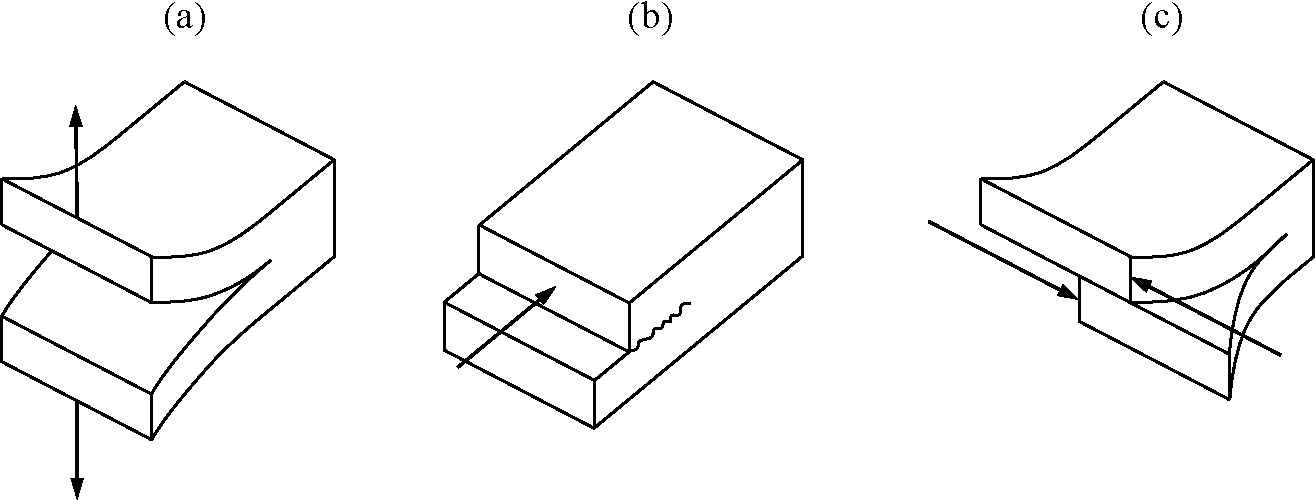
\includegraphics[scale=0.5]{fraturas.pdf}
	\end{center}
	\caption{\label{fig_grafico}Gráfico produzido em Excel e salvo como PDF (fonte: \citeonline[p. 24]{araujo2012})}
\end{figure}

% ---
\subsection{Figuras em \emph{minipages}}
% ---

\emph{Minipages} são usadas para inserir textos ou outros elementos em quadros
com tamanhos e posições controladas. Veja o exemplo da
\autoref{fig_minipage_imagem1} e da \autoref{fig_minipage_grafico2}.

\begin{figure}[htb]
 \label{teste}
 \centering
  \begin{minipage}{0.4\textwidth}
    \centering
    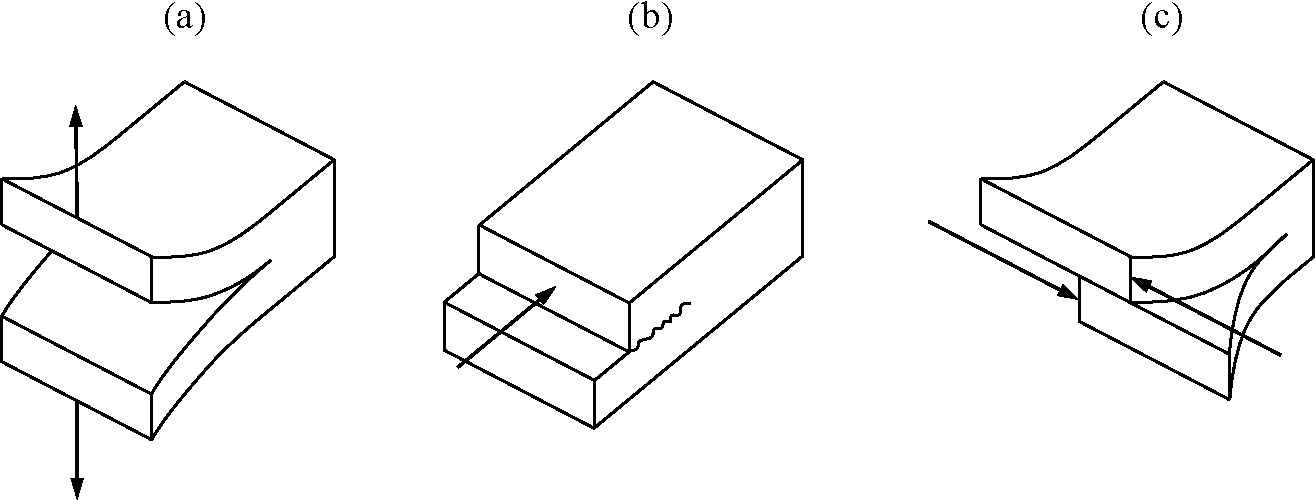
\includegraphics[scale=0.3]{fraturas.pdf}
    \caption{Imagem 1 da minipage} \label{fig_minipage_imagem1}
  \end{minipage}
  \hfill
  \begin{minipage}{0.4\textwidth}
    \centering
    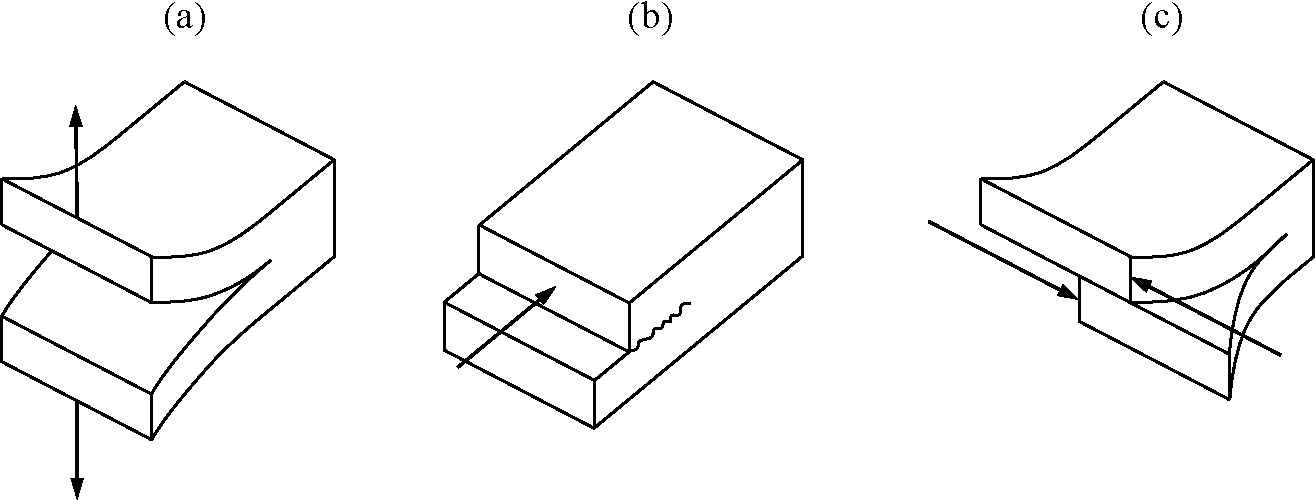
\includegraphics[scale=0.2]{fraturas.pdf}
    \caption{Gráfico 2 da minipage} \label{fig_minipage_grafico2}
  \end{minipage}
\end{figure}

Observe que, segundo a \citeonline[seções 4.2.1.10 e 5.8]{NBR14724:2011}, as
ilustrações devem sempre ter numeração contínua e única em todo o documento:

\begin{citacao}
Qualquer que seja o tipo de ilustração, sua identificação aparece na parte
superior, precedida da palavra designativa (desenho, esquema, fluxograma,
fotografia, gráfico, mapa, organograma, planta, quadro, retrato, figura,
imagem, entre outros), seguida de seu número de ordem de ocorrência no texto,
em algarismos arábicos, travessão e do respectivo título. Após a ilustração, na
parte inferior, indicar a fonte consultada (elemento obrigatório, mesmo que
seja produção do próprio autor), legenda, notas e outras informações
necessárias à sua compreensão (se houver). A ilustração deve ser citada no
texto e inserida o mais próximo possível do trecho a que se
refere. \cite[seções 5.8]{NBR14724:2011}
\end{citacao}

% ---
\section{Expressões matemáticas}
% ---

\index{expressões matemáticas}Use o ambiente \texttt{equation} para escrever
expressões matemáticas numeradas:

\begin{equation}
  \forall x \in X, \quad \exists \: y \leq \epsilon
\end{equation}

Escreva expressões matemáticas entre \$ e \$, como em $ \lim_{x \to \infty}
\exp(-x) = 0 $, para que fiquem na mesma linha.

Também é possível usar colchetes para indicar o início de uma expressão
matemática que não é numerada.

\[
\left|\sum_{i=1}^n a_ib_i\right|
\le
\left(\sum_{i=1}^n a_i^2\right)^{1/2}
\left(\sum_{i=1}^n b_i^2\right)^{1/2}
\]

Consulte mais informações sobre expressões matemáticas em
\url{https://github.com/abntex/abntex2/wiki/Referencias}.

% ---
\section{Enumerações: alíneas e subalíneas}
% ---

\index{alíneas}\index{subalíneas}\index{incisos}Quando for necessário enumerar
os diversos assuntos de uma seção que não possua título, esta deve ser
subdividida em alíneas \cite[4.2]{NBR6024:2012}:

\begin{alineas}

  \item os diversos assuntos que não possuam título próprio, dentro de uma mesma
  seção, devem ser subdivididos em alíneas; 
  
  \item o texto que antecede as alíneas termina em dois pontos;
  \item as alíneas devem ser indicadas alfabeticamente, em letra minúscula,
  seguida de parêntese. Utilizam-se letras dobradas, quando esgotadas as
  letras do alfabeto;

  \item as letras indicativas das alíneas devem apresentar recuo em relação à
  margem esquerda;

  \item o texto da alínea deve começar por letra minúscula e terminar em
  ponto-e-vírgula, exceto a última alínea que termina em ponto final;

  \item o texto da alínea deve terminar em dois pontos, se houver subalínea;

  \item a segunda e as seguintes linhas do texto da alínea começa sob a
  primeira letra do texto da própria alínea;
  
  \item subalíneas \cite[4.3]{NBR6024:2012} devem ser conforme as alíneas a
  seguir:

  \begin{alineas}
     \item as subalíneas devem começar por travessão seguido de espaço;

     \item as subalíneas devem apresentar recuo em relação à alínea;

     \item o texto da subalínea deve começar por letra minúscula e terminar em
     ponto-e-vírgula. A última subalínea deve terminar em ponto final, se não
     houver alínea subsequente;

     \item a segunda e as seguintes linhas do texto da subalínea começam sob a
     primeira letra do texto da própria subalínea.
  \end{alineas}
  
  \item no \abnTeX\ estão disponíveis os ambientes \texttt{incisos} e
  \texttt{subalineas}, que em suma são o mesmo que se criar outro nível de
  \texttt{alineas}, como nos exemplos à seguir:
  
  \begin{incisos}
    \item \textit{Um novo inciso em itálico};
  \end{incisos}
  
  \item Alínea em \textbf{negrito}:
  
  \begin{subalineas}
    \item \textit{Uma subalínea em itálico};
    \item \underline{\textit{Uma subalínea em itálico e sublinhado}}; 
  \end{subalineas}
  
  \item Última alínea com \emph{ênfase}.
  
\end{alineas}
% ---
\section{Espaçamento entre parágrafos e linhas}
% ---

\index{espaçamento!dos parágrafos}O tamanho do parágrafo, espaço entre a margem
e o início da frase do parágrafo, é definido por:

\begin{verbatim}
   \setlength{\parindent}{0cm}
   % (definição do PPGEC)
\end{verbatim}


\index{espaçamento!entre os parágrafos}O espaçamento entre um parágrafo e outro
pode ser controlado por meio do comando:

\begin{verbatim}
  \setlength{\parskip}{0.2cm}  % tente também \onelineskip
\end{verbatim}

\index{espaçamento!entre as linhas}O controle do espaçamento entre linhas é
definido por:

\begin{verbatim}
  \OnehalfSpacing       % espaçamento um e meio (padrão); 
  \DoubleSpacing        % espaçamento duplo
  \SingleSpacing        % espaçamento simples	
\end{verbatim}

Para isso, também estão disponíveis os ambientes:

\begin{verbatim}
  \begin{SingleSpace} ...\end{SingleSpace}
  \begin{Spacing}{hfactori} ... \end{Spacing}
  \begin{OnehalfSpace} ... \end{OnehalfSpace}
  \begin{OnehalfSpace*} ... \end{OnehalfSpace*}
  \begin{DoubleSpace} ... \end{DoubleSpace}
  \begin{DoubleSpace*} ... \end{DoubleSpace*} 
\end{verbatim}

Para mais informações, consulte \citeonline[p. 47-52 e 135]{memoir}.

% ---
\section{Inclusão de outros arquivos}\label{sec-include}
% ---

É uma boa prática dividir o seu documento em diversos arquivos, e não
apenas escrever tudo em um único. Esse recurso foi utilizado neste
documento. Para incluir diferentes arquivos em um arquivo principal,
de modo que cada arquivo incluído fique em uma página diferente, utilize o
comando:

\begin{verbatim}
   \include{documento-a-ser-incluido}
   % sem a extensão .tex
\end{verbatim}

Para incluir documentos sem quebra de páginas, utilize:

\begin{verbatim}
   \input{documento-a-ser-incluido}
   % sem a extensão .tex
\end{verbatim}

% ---
\section{Compilar o documento \LaTeX}
% ---

Geralmente os editores \LaTeX, como o
TeXlipse\footnote{\url{http://texlipse.sourceforge.net/}}, o
Texmaker\footnote{\url{http://www.xm1math.net/texmaker/}}, entre outros,
compilam os documentos automaticamente, de modo que você não precisa se
preocupar com isso.

No entanto, você pode compilar os documentos \LaTeX usando os seguintes
comandos, que devem ser digitados no \emph{Prompt de Comandos} do Windows ou no
\emph{Terminal} do Mac ou do Linux:

\begin{verbatim}
   pdflatex ARQUIVO_PRINCIPAL.tex
   bibtex ARQUIVO_PRINCIPAL.aux
   makeindex ARQUIVO_PRINCIPAL.idx 
   makeindex ARQUIVO_PRINCIPAL.nlo -s nomencl.ist -o
   ARQUIVO_PRINCIPAL.nls
   pdflatex ARQUIVO_PRINCIPAL.tex
   pdflatex ARQUIVO_PRINCIPAL.tex
\end{verbatim}

% ---
\section{Remissões internas}
% ---

Ao nomear a \autoref{tab-nivinv} e a \autoref{fig_circulo}, apresentamos um
exemplo de remissão interna, que também pode ser feita quando indicamos o
\autoref{cap_exemplos}, que tem o nome \emph{\nameref{cap_exemplos}}. O número
do capítulo indicado é \ref{cap_exemplos}, que se inicia à
\autopageref{cap_exemplos}\footnote{O número da página de uma remissão pode ser
obtida também assim:
\pageref{cap_exemplos}.}.
Veja a \autoref{sec-divisoes} para outros exemplos de remissões internas entre
seções, subseções e subsubseções.

O código usado para produzir o texto desta seção é:

\begin{verbatim}
Ao nomear a \autoref{tab-nivinv} e a \autoref{fig_circulo},
apresentamos umexemplo de remissão interna, que também pode
ser feita quando indicamos o \autoref{cap_exemplos}, que tem
o nome \emph{\nameref{cap_exemplos}}. O número do capítulo
indicado é \ref{cap_exemplos}, que se inicia à
\autopageref{cap_exemplos}\footnote{O número da página de uma
remissão pode ser obtida também assim:
\pageref{cap_exemplos}.}. Veja a \autoref{sec-divisoes}
para outros exemplos de remissões internas entre seções,
subseções e subsubseções.
\end{verbatim}

% ---
\section{Divisões do documento: seção}\label{sec-divisoes}
% ---

Esta seção testa o uso de divisões de documentos. Esta é a
\autoref{sec-divisoes}. Veja a \autoref{sec-divisoes-subsection}.

\subsection{Divisões do documento: subseção}\label{sec-divisoes-subsection}

Isto é uma subseção. Veja a \autoref{sec-divisoes-subsubsection}, que é uma
\texttt{subsubsection} do \LaTeX, mas é impressa chamada de ``subseção'' porque
no Português não temos a palavra ``subsubseção''.

\subsubsection{Divisões do documento: subsubseção}
\label{sec-divisoes-subsubsection}

Isto é uma subsubseção.

\subsubsection{Divisões do documento: subsubseção}

Isto é outra subsubseção.

\subsection{Divisões do documento: subseção}\label{sec-exemplo-subsec}

Isto é uma subseção.

\subsubsection{Divisões do documento: subsubseção}

Isto é mais uma subsubseção da \autoref{sec-exemplo-subsec}.


\subsubsubsection{Esta é uma subseção de quinto
nível}\label{sec-exemplo-subsubsubsection}

Esta é uma seção de quinto nível. Ela é produzida com o seguinte comando:

\begin{verbatim}
\subsubsubsection{Esta é uma subseção de quinto
nível}\label{sec-exemplo-subsubsubsection}
\end{verbatim}

\subsubsubsection{Esta é outra subseção de quinto nível}\label{sec-exemplo-subsubsubsection-outro}

Esta é outra seção de quinto nível.


\paragraph{Este é um parágrafo numerado}\label{sec-exemplo-paragrafo}

Este é um exemplo de parágrafo nomeado. Ele é produzida com o comando de
parágrafo:

\begin{verbatim}
\paragraph{Este é um parágrafo
nomeado}\label{sec-exemplo-paragrafo}
\end{verbatim}

A numeração entre parágrafos numeradaos e subsubsubseções são contínuas.

\paragraph{Esta é outro parágrafo numerado}\label{sec-exemplo-paragrafo-outro}

Esta é outro parágrafo nomeado.

% ---
\section{Este é um exemplo de nome de seção longo. Ele deve estar
alinhado à esquerda e a segunda e demais linhas devem iniciar logo abaixo da
primeira palavra da primeira linha}
% ---

Isso atende à norma \citeonline[seções de 5.2.2 a 5.2.4]{NBR14724:2011} 
 e \citeonline[seções de 3.1 a 3.8]{NBR6024:2012}.

% ---
\section{Diferentes idiomas e hifenizações}
\label{sec-hifenizacao}
% ---

Para usar hifenizações de diferentes idiomas, inclua nas opções do documento o
nome dos idiomas que o seu texto contém. Por exemplo (para melhor
visualização, as opções foram quebras em diferentes linhas):

\begin{verbatim}
\documentclass[
	12pt,
	openright,
	twoside,
	a4paper,
	english,
	french,
	spanish,
	brazil
	]{abntex2}
\end{verbatim}

O idioma português-brasileiro (\texttt{brazil}) é incluído automaticamente pela
classe \textsf{abntex2}. Porém, mesmo assim a opção \texttt{brazil} deve ser
informada como a última opção da classe para que todos os pacotes reconheçam o
idioma. Vale ressaltar que a última opção de idioma é a utilizada por padrão no
documento. Desse modo, caso deseje escrever um texto em inglês que tenha
citações em português e em francês, você deveria usar o preâmbulo como abaixo:

\begin{verbatim}
\documentclass[
	12pt,
	openright,
	twoside,
	a4paper,
	french,
	brazil,
	english
	]{abntex2}
\end{verbatim}

A lista completa de idiomas suportados, bem como outras opções de hifenização,
estão disponíveis em \citeonline[p.~5-6]{babel}.

Exemplo de hifenização em inglês\footnote{Extraído de:
\url{http://bit.ly/2PHmwhd}}:

\begin{otherlanguage*}{english}
\textit{Text in English language. This environment switches all language-related
definitions, like the language specific names for figures, tables etc. to the other
language. The starred version of this environment typesets the main text
according to the rules of the other language, but keeps the language specific
string for ancillary things like figures, in the main language of the document.
The environment hyphenrules switches only the hyphenation patterns used; it can
also be used to disallow hyphenation by using the language name
`nohyphenation'.}
\end{otherlanguage*}

Exemplo de hifenização em francês\footnote{Extraído de:
\url{http://bit.ly/3476ke9}}:

\begin{otherlanguage*}{french}
\textit{Texte en français. Pas question que Twitter ne vienne faire une
concurrence déloyale à la traditionnelle fumée blanche qui marque l'élection
d'un nouveau pape. Pour éviter toute fuite précoce, le Vatican a donc pris un
peu d'avance, et a déjà interdit aux cardinaux qui prendront part au vote
d'utiliser le réseau social, selon Catholic News Service. Une mesure valable
surtout pour les neuf cardinaux – sur les 117 du conclave – pratiquants très
actifs de Twitter, qui auront interdiction pendant toute la période de se
connecter à leur compte.}
\end{otherlanguage*}

Pequeno texto em espanhol\footnote{Extraído de:
\url{http://bit.ly/2PvgcsP}}:

\foreignlanguage{spanish}{\textit{Decenas de miles de personas ovacionan al pontífice en su
penúltimo ángelus dominical, el primero desde que anunciase su renuncia. El Papa se
centra en la crítica al materialismo}}.

O idioma geral do texto por ser alterado como no exemplo seguinte:

\begin{verbatim}
  \selectlanguage{english}
\end{verbatim}

Isso altera automaticamente a hifenização e todos os nomes constantes de
referências do documento para o idioma inglês. Consulte o manual da classe
\cite{abntex2classe} para obter orientações adicionais sobre internacionalização de
documentos produzidos com \abnTeX.

A \autoref{sec-citacao} descreve o ambiente \texttt{citacao} que pode receber
como parâmetro um idioma a ser usado na citação.

% ---
\section{Consulte o manual da classe \textsf{abntex2}}
% ---

Consulte o manual da classe \textsf{abntex2} \cite{abntex2classe} para uma
referência completa das macros e ambientes disponíveis. 

Além disso, o manual possui informações adicionais sobre as normas ABNT
observadas pelo \abnTeX\ e considerações sobre eventuais requisitos específicos
não atendidos, como o caso da \citeonline[seção 5.2.2]{NBR14724:2011}, que
especifica o espaçamento entre os capítulos e o início do texto, regra
propositalmente não atendida pelo presente modelo.

% ---
\section{Referências bibliográficas}
% ---

A formatação das referências bibliográficas conforme as regras da ABNT são um
dos principais objetivos do \abnTeX. Consulte os manuais
\citeonline{abntex2cite} e \citeonline{abntex2cite-alf} para obter informações
sobre como utilizar as referências bibliográficas.

%-
\subsection{Acentuação de referências bibliográficas}
%-

Normalmente não há problemas em usar caracteres acentuados em arquivos
bibliográficos (\texttt{*.bib}). Porém, como as regras da ABNT fazem uso quase
abusivo da conversão para letras maiúsculas, é preciso observar o modo como se
escreve os nomes dos autores. Na ~\autoref{tabela-acentos} você encontra alguns
exemplos das conversões mais importantes. Preste atenção especial para `ç' e `í'
que devem estar envoltos em chaves. A regra geral é sempre usar a acentuação
neste modo quando houver conversão para letras maiúsculas.

\begin{table}[htbp]
\caption{Tabela de conversão de acentuação.}
\label{tabela-acentos}

\begin{center}
\begin{tabular}{ll}\hline\hline
acento & \textsf{bibtex}\\
à á ã & \verb+\`a+ \verb+\'a+ \verb+\~a+\\
í & \verb+{\'\i}+\\
ç & \verb+{\c c}+\\
\hline\hline
\end{tabular}
\end{center}
\end{table}


% ---
\section{Precisa de ajuda?}
% ---

Consulte a FAQ com perguntas frequentes e comuns no portal do \abnTeX:
\url{https://github.com/abntex/abntex2/wiki/FAQ}.

Inscreva-se no grupo de usuários \LaTeX:
\url{http://groups.google.com/group/latex-br}, tire suas dúvidas e ajude
outros usuários.

Participe também do grupo de desenvolvedores do \abnTeX:
\url{http://groups.google.com/group/abntex2} e faça sua contribuição à
ferramenta.

% ---
\section{Você pode ajudar?}
% ---

Sua contribuição é muito importante! Você pode ajudar na divulgação, no
desenvolvimento e de várias outras formas. Veja como contribuir com o \abnTeX\
em \url{https://github.com/abntex/abntex2/wiki/Como-Contribuir}.

% ---
\section{Quer ajudar a customizar os modelos do \abnTeX\ para o PPGEC-UFRGS?}
% ---

Me ajude reportando erros e otimizações na customização\footnote{me manda um e-mail: augusto.borges@ufrgs.br} e, se quiser ir além, veja como customizar o \abnTeX\ em:
\url{https://github.com/abntex/abntex2/wiki/ComoCustomizar}.		% Capítulo 3: Nome
% %%%%%%%%%%%%%%%%%%%%%%%%%%%%%%%%%%%%%%%%%%%%%%%%%%%%%%%%%%%%%%%%%%%%%%%%%%%%%%%%%
%
%	cap#.tex 
%  -----------
%
%	Neste arquivo você escreve o capítulo. Deve sempre iniciar com o ambiente
%	\chapter{Nome do Capitulo}
%
% %%%%%%%%%%%%%%%%%%%%%%%%%%%%%%%%%%%%%%%%%%%%%%%%%%%%%%%%%%%%%%%%%%%%%%%%%%%%%%%%%
%
\chapter{Conteúdos específicos do modelo de trabalho no modelo}\label{cap_trabalho_academico}
% ----------------------------------------------------------

\section{Quadros}

Este modelo vem com o ambiente \texttt{quadro} e impressão de Lista de quadros 
configurados por padrão. Verifique um exemplo de utilização:

\begin{quadro}[htb]
\caption{\label{quadro_exemplo}Exemplo de quadro (fonte: Autor)}
\begin{tabular}{|c|c|c|c|}
	\hline
	\textbf{Pessoa} & \textbf{Idade} & \textbf{Peso} & \textbf{Altura} \\ \hline
	Marcos & 26    & 68   & 178    \\ \hline
	Ivone  & 22    & 57   & 162    \\ \hline
	...    & ...   & ...  & ...    \\ \hline
	Sueli  & 40    & 65   & 153    \\ \hline
\end{tabular}
\end{quadro}

Este parágrafo apresenta como referenciar o quadro no texto, requisito
obrigatório da ABNT. 
Primeira opção, utilizando \texttt{autoref}: Ver o \autoref{quadro_exemplo}. 
Segunda opção, utilizando  \texttt{ref}: Ver o Quadro \ref{quadro_exemplo}.		% Capítulo 4: Nome
% %%%%%%%%%%%%%%%%%%%%%%%%%%%%%%%%%%%%%%%%%%%%%%%%%%%%%%%%%%%%%%%%%%%%%%%%%%%%%%%%%
%
%	cap#.tex 
%  -----------
%
%	Neste arquivo você escreve o capítulo. Deve sempre iniciar com o ambiente
%	\chapter{Nome do Capitulo}
%
% %%%%%%%%%%%%%%%%%%%%%%%%%%%%%%%%%%%%%%%%%%%%%%%%%%%%%%%%%%%%%%%%%%%%%%%%%%%%%%%%%
%
\chapter{Novo Capítulo}
% ----------------------------------------------------------

% ---
\section{Oi, tudo bom?}
% ---

Minha terra tem palmeiras, onde canta o sabiá... \autoref{apendicea}
		% Capítulo 5: Nome
%\include{./chap/cap6}		% Capítulo 6: Nome
%\include{./chap/cap7}		% Capítulo 7: Nome
%
% Carrega configuração dos elementos pós textuais
\postextualconfig
%
% Imprimir referencias
\bibliography{./bib/referencias}
%
% Imprimir apêndices
% Comente os comandos abaixo na ausência de apêndices
\imprimircapaapendices
% %%%%%%%%%%%%%%%%%%%%%%%%%%%%%%%%%%%%%%%%%%%%%%%%%%%%%%%%%%%%%%%%%%%%%%%%%%%%%%%%%
%
%	ape#.tex 
%  -----------
%
%	Neste arquivo você escreve o anexo. Deve sempre iniciar o ambiente \chapter.
%
%
% %%%%%%%%%%%%%%%%%%%%%%%%%%%%%%%%%%%%%%%%%%%%%%%%%%%%%%%%%%%%%%%%%%%%%%%%%%%%%%%%%
%
\chapter{Quisque libero justo}
\label{apendicea}

\lipsum[50]	
% %%%%%%%%%%%%%%%%%%%%%%%%%%%%%%%%%%%%%%%%%%%%%%%%%%%%%%%%%%%%%%%%%%%%%%%%%%%%%%%%%
%
%	ape#.tex 
%  -----------
%
%	Neste arquivo você escreve o anexo. Deve sempre iniciar o ambiente \chapter.
%
%
% %%%%%%%%%%%%%%%%%%%%%%%%%%%%%%%%%%%%%%%%%%%%%%%%%%%%%%%%%%%%%%%%%%%%%%%%%%%%%%%%%
%
\chapter{Nullam elementum urna vel imperdiet sodales elit ipsum pharetra ligula
	ac pretium ante justo a nulla curabitur tristique arcu eu metus}

\lipsum[55-57]
% %%%%%%%%%%%%%%%%%%%%%%%%%%%%%%%%%%%%%%%%%%%%%%%%%%%%%%%%%%%%%%%%%%%%%%%%%%%%%%%%%
%
%	ape#.tex 
%  -----------
%
%	Neste arquivo você escreve o anexo. Deve sempre iniciar o ambiente \chapter.
%
%
% %%%%%%%%%%%%%%%%%%%%%%%%%%%%%%%%%%%%%%%%%%%%%%%%%%%%%%%%%%%%%%%%%%%%%%%%%%%%%%%%%
%
\chapter{Exemplo de apêndice com subsecção}


\section{Seção de Apêndice C}



\section{Seção de Apêndice C}



\subsection{Subseção de Apêndice C}
%
% Imprimir anexos
% Comente os comandos abaixo na ausência de anexos
\imprimircapaanexos
% %%%%%%%%%%%%%%%%%%%%%%%%%%%%%%%%%%%%%%%%%%%%%%%%%%%%%%%%%%%%%%%%%%%%%%%%%%%%%%%%%
%
%	ane#.tex 
%  -----------
%
%	Neste arquivo você escreve o anexo. Deve sempre iniciar o ambiente \chapter.
%
%
% %%%%%%%%%%%%%%%%%%%%%%%%%%%%%%%%%%%%%%%%%%%%%%%%%%%%%%%%%%%%%%%%%%%%%%%%%%%%%%%%%
%

\chapter{Morbi ultrices rutrum lorem.}

\lipsum[30]	
% %%%%%%%%%%%%%%%%%%%%%%%%%%%%%%%%%%%%%%%%%%%%%%%%%%%%%%%%%%%%%%%%%%%%%%%%%%%%%%%%%
%
%	ane#.tex 
%  -----------
%
%	Neste arquivo você escreve o anexo. Deve sempre iniciar o ambiente \chapter.
%
%
% %%%%%%%%%%%%%%%%%%%%%%%%%%%%%%%%%%%%%%%%%%%%%%%%%%%%%%%%%%%%%%%%%%%%%%%%%%%%%%%%%
%
\chapter{Anexo B - Cras non urna sed feugiat cum sociis natoque penatibus et magnis dis
	parturient montes nascetur ridiculus mus}

\lipsum[31]
% %%%%%%%%%%%%%%%%%%%%%%%%%%%%%%%%%%%%%%%%%%%%%%%%%%%%%%%%%%%%%%%%%%%%%%%%%%%%%%%%%
%
%	ane#.tex 
%  -----------
%
%	Neste arquivo você escreve o anexo. Deve sempre iniciar o ambiente \chapter.
%
%
% %%%%%%%%%%%%%%%%%%%%%%%%%%%%%%%%%%%%%%%%%%%%%%%%%%%%%%%%%%%%%%%%%%%%%%%%%%%%%%%%%
%
\chapter{Fusce facilisis lacinia dui}

\lipsum[32]
%
% Imprimir anexos em pdf: \imprimiranexopdf{nome do arquivo}{título do anexo}{primeirapagina}{proximaspaginas}
% Comente oo comando abaixo para remover páginas com símbolos em latex
\imprimiranexopdf{./pos/latex_symbols}{Símbolos matemáticos}{1}{2-}
%
%
\end{document}

